\documentclass{article}
\setlength{\parskip}{5pt} % esp. entre párrafos
\setlength{\parindent}{0pt} % esp. al inicio de un párrafo
\usepackage{amsmath} % mates
\usepackage{url} % que las URLs se vean lindos
\usepackage[top=25mm,left=20mm,right=20mm,bottom=25mm]{geometry} % márgenes

\usepackage[utf8]{inputenc}
\usepackage[margin=1in]{geometry}
\usepackage{amsmath,amsfonts,amssymb,mathtools}
\usepackage{graphicx,float}
\usepackage{algorithmic}
\usepackage{minted}
\usepackage{subcaption}
\usepackage{multicol}
\usepackage{listings}
\usepackage{xcolor}
\usepackage[sort&compress,numbers]{natbib} % referencias
\usepackage{minted}
\usepackage{hyperref} % ligas de URLs
\usepackage{graphicx} % poner figuras
\usepackage[spanish]{babel} % otros idiomas
\usepackage{listings}
\author{Raul L.} % author
\title{Pr\'{a}ctica 5: método Monte-Carlo} %título
\date{\today}
\begin{document} % inicia contenido

\maketitle % cabecera


\section{Introducci\'{o}n}\label{intro} % sección y etiqueta



El método Monte Carlo es idóneo para situaciones en las cuales algún valor o alguna distribución no se conoce y resulta complicado de determinar de manera analítica. Siguiendo los ejemplos de Kurt, paralelicemos algunos casos sencillos en esta práctica.
Supongamos que se ocupa conocer el valor de una integral que no se nos antoja resolver para nada, como, por ejemplo

\[ \int_{3}^{7} f(x) \,dx \] para
\[f(x) = \frac {1}{exp(x) + exp(-x)}\]
Por suerte, 2$f(x)/ \pi$ es una función de distribución valida, ya que
\[ \int_{-\infty}^{\infty}\frac{2}{\pi} f(x) \,dx = 1\]
Este hecho nos permite generar números pseudoaleatorios con la distribución 	g(x) = 2 f(x)/ $\pi$, \\ así \ estimar \[ \int_{3}^{7} g(x) \,dx \]
\ y de ahí normalizar el estimado para que sea \[\int_{3}^{7} f(x) \,dx\] \\
Se puede comparar con el resultado aproximado de Wolfram Alpha, 0.048834, para llegar a una satisfacción que no estemos completamente mal. Se debe notar que cada ejecución dará un resultado distinto ya que es una muestra pseudoaleatoria \citep{ejemplo}.

\section{Objetivo}
Estudia estadísticamente la convergencia de la precisión del estimado del integral con en método Monte Carlo, comparando con el valor producido por Wolfram Alpha, en términos del (1) error absoluto, (2) error cuadrado y (3) cantidad de decimales correctos, aumentando el tamaño de muestra \citep{ejemplo2}.

\newpage



\section{C\'{o}digo}
Para este código se utilizaron un numero alto de repeticiones  repeticiones para cada pedazo, esta cantidad fue con la que se observó que se podía llegar a cuatro decimales de precisión. No se pudo llegar a observar los resultados con más repeticiones por falta de poder de procesamiento.

 Código en Python 

\url{https://github.com/satuelisa/Simulation/blob/master/MonteCarlo/rng.py}

**Código creado en Python**

\url{https://github.com/Raullr28/Resultados/blob/main/P4/codigo_celdas.py}
\renewcommand{\listingscaption}{Código}

\begin{listing}[H]
\begin{minted}{python}
vg = np.vectorize(g)
X = np.arange(-8, 8, 0.05) # ampliar y refinar
Y = vg(X) # mayor eficiencia
correcto= 0.04883411112604931084064237
print("correcto",correcto)
desde = 2.96 
hasta = 7
pdz = (700,5000,10000,80000,300000,1000000)#,5000000)#numero de n para estimar valor
repeticiones = 200
result = {"Estimado": [], "abs": [], "cuad": [], "dec": []}
dec = {"cero": [], "uno": [], "dos": [], "tres": [], "cuatro": [], "cinco": []}
ABS, CUAD = [],[]
for pedazo in pdz:
    print("############## pedazos:",pedazo,"######################")
    absoluto=[]
    cuadrado=[]
    dec_corr=[]
    for i in range(repeticiones):
        generador = GeneralRandom(np.asarray(X), np.asarray(Y))
        V = generador.random(pedazo)[0]
        montecarlo = ((V >= desde) & (V <= hasta))
        integral = sum(montecarlo) / (pedazo)
        estimado=(pi / 2) * integral
        absoluto.append(abs(correcto - estimado))
        cuadrado.append(((correcto - estimado)**2))
        dec_corr.append(decimales(correcto, estimado))#regresa cuantos decimales hubo semejantes


  \end{minted}
  \label{lst:fibo}
  \caption{Representa la automatización para variar el pedo.}
\end{listing}
\renewcommand{\listingscaption}{Código}
\begin{listing}[H]

\begin{minted}{python}
 
def g(x):
    return (2  / (pi * (exp(x) + exp(-x))))

def decimales(real, obtenido):
    contador=-2 #omite el 0 y el punto . del conteo
    real, obtenido= (str(real)), (str(obtenido))# convierte para leer cada valor
    obtenido=obtenido[:(len(real))]# recorte para mismo tamaño
    largo=min([len(real),len(obtenido)])
    for i in range(largo):
        if real[i] == obtenido[i]:
            contador=contador+1
        else:
            break
    return(contador)
  \end{minted}
  \label{lst:fibo}
  \caption{Representación función decimales.}
\end{listing}

% Computational Results
\section{Resultados}
En las figuras se muestra la probabilidad que existió en cada una de los diferentes partes con un número de repeticiones de 100, esto se realizó para poder dar un resultado estadístico ya que con esto podíamos comparar la probabilidad de encontrar los decimales correctos en cada una de las diferentes partes.

\begin{figure}[H]
\centering
\begin{subfigure}[Absoluto]{0.40\linewidth}
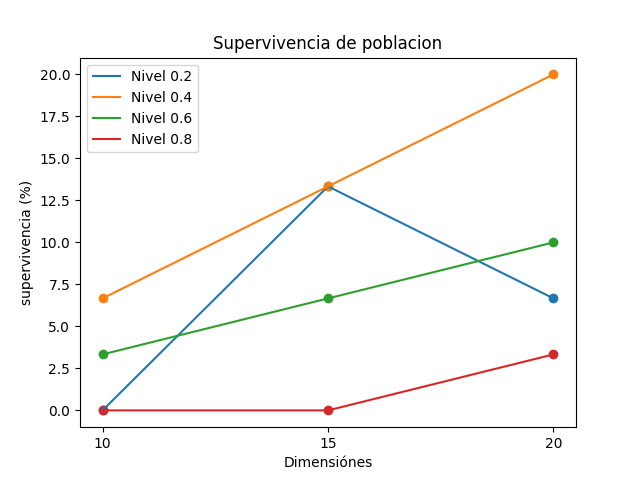
\includegraphics[width=\linewidth]{imagenes/Figure_1.png}
\caption{}
\end{subfigure}
\begin{subfigure}[Cuadrado]{0.40\linewidth}
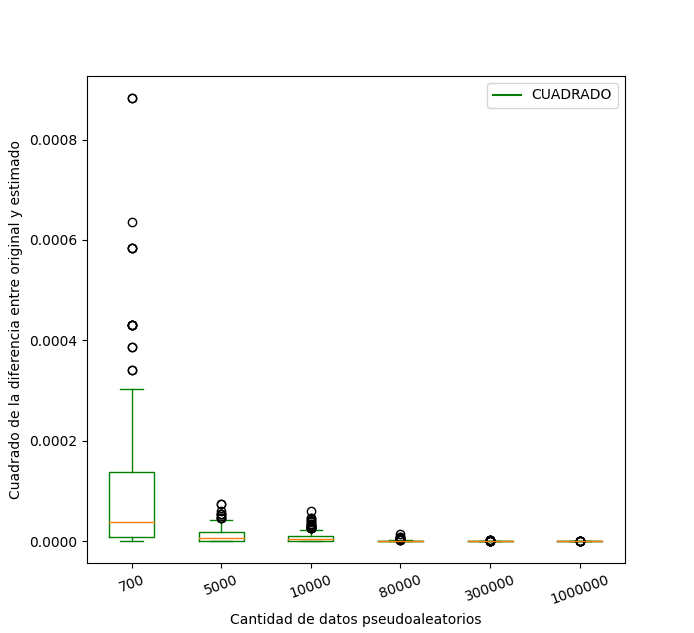
\includegraphics[width=\linewidth]{imagenes/Figure_2.png}
\caption{}
\end{subfigure}
\caption{Grafica comparativa.}
\label{fig:westminster}
\end{figure}

\begin{figure}[H]
\centering
\begin{subfigure}[b]{0.50\linewidth}
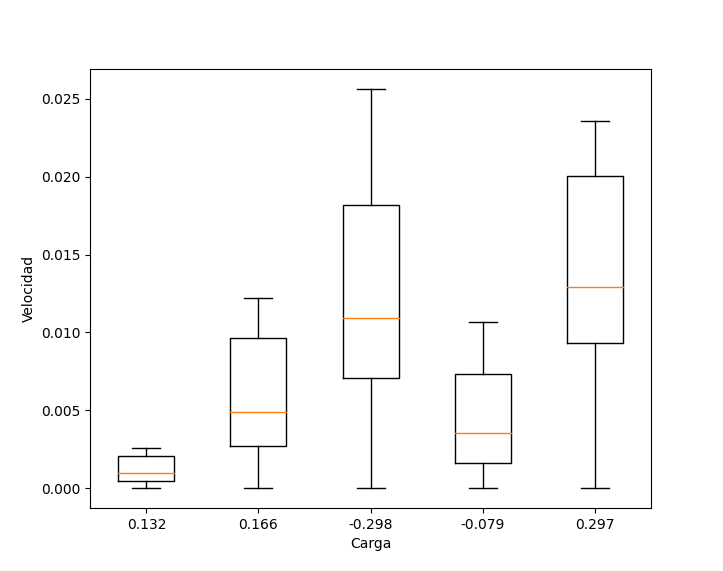
\includegraphics[width=\linewidth]{imagenes/Figure_3.png}
\caption{}
\end{subfigure}
\caption{Grafica estadística de porcentaje.}
\label{fig:westminster}
\end{figure}


\section{Reto 1}
El primer reto es realizar lo mismo para la estimación del valor de $ \Pi$   de  Kurt  \citep{kurt}.

 \begin{figure}[H]
\centering
\begin{subfigure}[Puntos dentro del circulo]{0.40\linewidth}
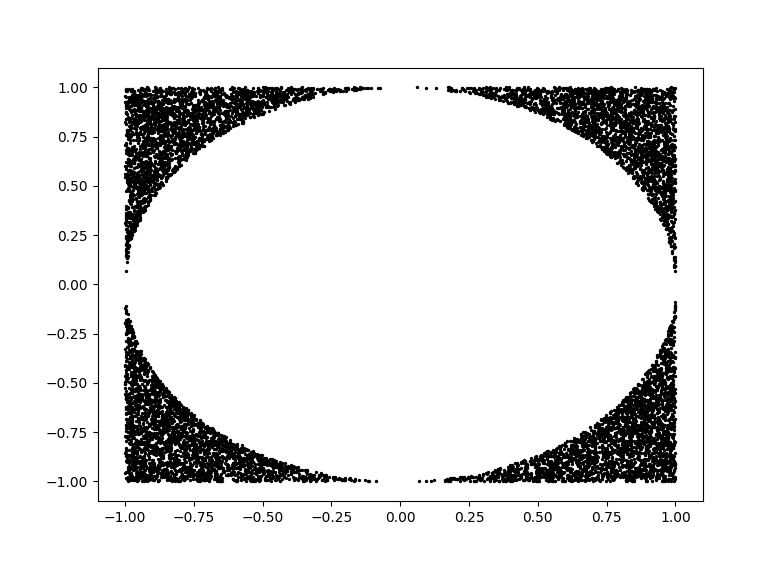
\includegraphics[width=\linewidth]{imagenes/figura4.png}
\caption{ciclo 0}
\end{subfigure}
\begin{subfigure}[Puntos fuera del circulo]{0.40\linewidth}

\includegraphics[width=\linewidth]{imagenes/figura5.png}
\caption{ciclo 3}
\end{subfigure}
\caption{Imagen de crecimiento aleatorio de puntos.}
\label{fig:westminster}
\end{figure}

\section{Resultados}
 \begin{figure}[H]
\centering
\begin{subfigure}[b]{0.40\linewidth}
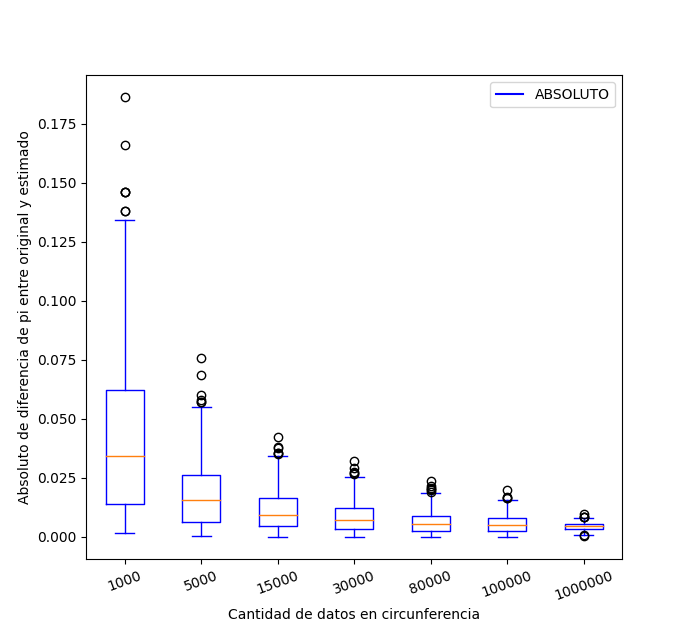
\includegraphics[width=\linewidth]{imagenes/Figure_1reto.png}
\caption{ciclo 6}
\end{subfigure}
\begin{subfigure}[b]{0.40\linewidth}
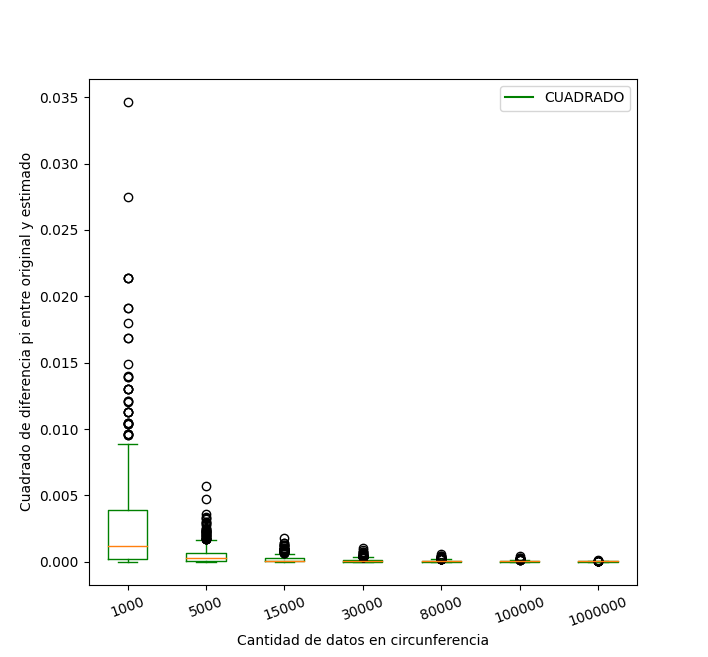
\includegraphics[width=\linewidth]{imagenes/Figure_2reto1.png}
\caption{ciclo 9}
\end{subfigure}
\caption{Imagen de crecimiento aleatorio de semillas.}
\label{fig:westminster}
\end{figure}

\begin{figure}[H]
\centering
\begin{subfigure}[b]{0.40\linewidth}
\includegraphics[width=\linewidth]{imagenes/Figure_3reto1.png}
\caption{ciclo 15}
\end{subfigure}
\label{fig:westminster}
\end{figure}

 \section{Conclusión}

Se demostró que aumentando el numero de repeticiones se podría llegar a tener un porcentaje alto de números decimales correctos.

 \bibliography{biblio.bib}
 \bibliographystyle{plainnat}

 \end{document}
